% ============================================================================
% example_figures.tex — v3.4 smoke test for the FIGURE / LISTING / QUOTE setup.
% Inputs the REAL preamble.tex, so compiling it tests the actual environment.
%
%   lualatex -interaction=nonstopmode example_figures.tex   (run via build.sh)
%   python3 ../scripts/check_bidi_figures.py example_figures.tex   # must be clean
%
% By design it exercises every v4 edge that hides a bug, so a regression is
% VISIBLE on the page rather than silent:
%   - a TikZ node mixing Hebrew + Latin + parens (must read forward, not UPC)
%   - bare-Latin TikZ nodes inside the LTR island (Datapath, Control)
%   - a code listing INSIDE a box (must sit inside the border, not spill left)
%   - a \code{} frametitle with a trailing ';' (must stay at the end)
%   - gershayim ״ quotes (must be symmetric, not “ ”)
%   - a Hebrew label under a brace via \text{\h{...}} (math-mode escape)
% ============================================================================
% ============================================================================
% preamble.tex — tested LuaLaTeX preamble for Hebrew + math + figures PDFs (v3.23)
% Battle-tested: compiled an 80-page Hebrew quantum-computing summary AND a
% 197-page Hebrew computer-architecture anthology (TikZ diagrams, code listings,
% colored boxes) — both with 0 missing characters.
%
% Usage in your document:
%   % ============================================================================
% preamble.tex — tested LuaLaTeX preamble for Hebrew + math + figures PDFs (v3.23)
% Battle-tested: compiled an 80-page Hebrew quantum-computing summary AND a
% 197-page Hebrew computer-architecture anthology (TikZ diagrams, code listings,
% colored boxes) — both with 0 missing characters.
%
% Usage in your document:
%   % ============================================================================
% preamble.tex — tested LuaLaTeX preamble for Hebrew + math + figures PDFs (v3.23)
% Battle-tested: compiled an 80-page Hebrew quantum-computing summary AND a
% 197-page Hebrew computer-architecture anthology (TikZ diagrams, code listings,
% colored boxes) — both with 0 missing characters.
%
% Usage in your document:
%   \input{preamble.tex}     % (or paste these lines at the top)
%   \begin{document}  ...  \end{document}
%
% Compile with:  lualatex -interaction=nonstopmode doc.tex   (twice, for TOC)
% Requires the Hebrew fonts installed (run scripts/setup_fonts.sh first).
%
% SHORT doc (exam + solution): change `report` -> `article`.
% STUDY doc meant to be read/annotated: 12pt + \linespread{1.3} below are
%   deliberate readability choices (NOT padding) — keep or trim to taste.
% ============================================================================
\documentclass[12pt]{report}          % 12pt: readable for a study guide; 11pt is fine too
\usepackage[no-math]{fontspec}        % (1) ★ no-math — THE critical line (see recipe.md)
\usepackage[bidi=basic]{babel}        % (2) RTL handling built into the engine
\babelprovide[import,main]{hebrew}    % (3) Hebrew = main language, default RTL
\babelprovide[import]{english}        % (4) English secondary, for correct LTR runs
% Latin fallback registered BEFORE \babelfont so a lone English word in Hebrew
% prose does not tofu. Fonts resolved by FAMILY NAME (portable; no hard path).
\directlua{luaotfload.add_fallback("hebfb",{"DejaVuSerif:mode=node;"})}
% v3.22: Frank Ruhl Libre ships NO italic face. Instead of silently-upright
% \emph (v<=3.20) or bold-as-emphasis (v3.21), synthesize a slanted face with
% FakeSlant — real, VISIBLE italic emphasis with correct \emph nesting
% semantics (inner \emph toggles back upright). Verified empirically at
% 300dpi: slant clearly visible, 0 errors, 0 missing glyphs.
\babelfont{rm}[RawFeature={fallback=hebfb},
  ItalicFont={Frank Ruhl Libre}, ItalicFeatures={FakeSlant=0.22},
  BoldItalicFont={Frank Ruhl Libre Bold}, BoldItalicFeatures={FakeSlant=0.22}
  ]{Frank Ruhl Libre}
\babelfont{sf}[RawFeature={fallback=hebfb}]{Heebo}
\babelfont{tt}[RawFeature={fallback=hebfb}]{DejaVu Sans Mono}

\usepackage{amsmath,amssymb,mathtools}
\usepackage[margin=2.3cm,headheight=14pt]{geometry}
\linespread{1.3}                      % readable line spacing for study/annotation docs
\usepackage{xcolor}
\usepackage{mdframed}
\usepackage{listings}                 % code listings (assembly / C / pseudo-code)
\usepackage{tikz}
\usetikzlibrary{arrows.meta,positioning,calc,shapes.geometric,fit,backgrounds}
\usepackage{pgfplots}\pgfplotsset{compat=1.18}
\usepackage{quantikz}                 % quantum circuits (remove if unused)
\usepackage{booktabs}
\usepackage{longtable}
\usepackage{array}
\usepackage{float}                    % [H] = place table exactly here (reference doc: no drifting)
\usepackage{enumitem}
\usepackage{needspace}

% ============================================================================
% ★★ v3.4 — THE DIRECTION-ISOLATION TRIO (the heart of mixing Hebrew + Latin)
% Mental model:
%   \h{...}    Hebrew (RTL) island      — Hebrew text inside an LTR context
%                                          (TikZ nodes, the english `tikzpic`).
%   \en{...}   English (LTR) isolate    — Latin text / parentheses inside a
%                                          Hebrew (RTL) context. KEEPS PARENS
%                                          AND ORDER CORRECT.
%   \code{...} \en + monospace          — code inside Hebrew / inside a frametitle.
% CRITICAL: never wrap Latin in \h{} (it is for HEBREW). Inside a TikZ node,
% Latin in \h{} renders REVERSED (Datapath->htapataD, CPU->UPC) and parens
% mirror. Isolate every Latin/paren chunk with \en{} or \code{}. See
% references/figures-boxes-listings.md.
% ---- TEXT INSIDE MATH (v3.8) ----------------------------------------------
% Put ANY text that sits inside math in a \text{}. The ONLY thing that is
% invalid in math is a bare \h/\en (= \foreignlanguage) used DIRECTLY, outside
% \text -> "\rmfamily invalid in math mode". Inside \text:
%   Hebrew label           -> \text{...}            (bare Hebrew renders fine;
%                              \h is OPTIONAL/harmless: \text{\h{...}} also works
%                              and both render identically + scale in scripts)
%   plain Latin word        -> \text{...}            (no marker needed)
%   Latin WITH ( ) or [ ]   -> \text{\en{...}}       (\en forces LTR; a plain
%                              \text mirrors the parens in RTL -> "Spec (TNR(" )
%   f(Hebrew/text arg)      -> \text{f}(\text{...})  -- keep the parens at MATH
%                              level, NOT \text{f(arg)} (parens inside the box mirror)
%   code in math            -> \mathtt{...}  (or \texttt{}, math-guarded below)
% NEVER write \en{...} or \h{...} straight into $...$ / \[..\] (outside \text);
% always via \text{}. (\mbox{...} also works but does not scale in scripts.)
% ============================================================================
\newcommand{\h}[1]{\foreignlanguage{hebrew}{#1}}
\newcommand{\en}[1]{\foreignlanguage{english}{#1}}

% ============================================================================
% ★★ — fixes for defects that are INVISIBLE in the log and in the checks
% and only surface on a VISUAL RENDER of the PDF. (Each verified empirically.)
% ----------------------------------------------------------------------------
% v3.22: \emph is now REAL slanted emphasis (FakeSlant italic face defined on
% the \babelfont{rm} line above), replacing the v3.21 \emph->\textbf hack: it
% preserves \emph's toggle semantics and keeps bold free for its own role.
% Prefer bold-as-emphasis for your doc? one line: \renewcommand{\emph}[1]{\textbf{#1}}
% page number: force the digits LTR so they never reverse (18 -> 81) in the RTL
%   footer. That reversal is a NON-DETERMINISTIC bidi glitch (observed once in
%   ~80 pp); this LuaLaTeX build is not byte-reproducible, so the defensive
%   LTR wrap is the only reliable guard. Latin digits are always LTR anyway.
\renewcommand{\thepage}{\foreignlanguage{english}{\arabic{page}}}
% emergencystretch: Hebrew does not hyphenate, so an unbreakable LTR island
%   (\en{...} / an inline math run) landing at the margin can leave a small
%   (~2-13pt) overfull with no legal breakpoint. This rescues ONLY those
%   inline-prose tie-breaks; it is a ceiling used only on offending lines and
%   does NOT touch display-math / listing / table overflow (those still surface
%   in the log for the content-level overflow pass). Verified: baseline overfull
%   -> 0 with this set, with no change to pagination or underfull.
\setlength{\emergencystretch}{3em}
% em-dash: --- does NOT become — under Frank Ruhl (the font lacks tlig; verified
%   the width is identical with/without Ligatures=TeX, while the mechanism works
%   on Latin Modern). TYPE THE CHARACTER — (U+2014) DIRECTLY; likewise – (U+2013).
%   check_bidi_figures.py flags a --/--- that is adjacent to Hebrew.
% ============================================================================

% ---- STRUCTURAL DIRECTION-SAFETY for \texttt (v3.7) -------------------------
% A parenthesis, bracket, or $ INSIDE \texttt{} mirrors/migrates in RTL prose
% (MIPS 0($s0)->"(s0$)0", $rs->"rs$", arr[i]->"[arr[i") because \texttt sets the
% font but NOT the direction. Redefining \texttt to LTR-isolate its content fixes
% the WHOLE class at once (parens, brackets, $) so plain \texttt{lw $t0,0($s0)}
% is safe — no need to remember \code{}. Guarded by \ifmmode because
% \foreignlanguage is invalid in math (there, plain monospace is already LTR).
% NB: \texttt{Hebrew} stays tofu — the monospace font has no Hebrew anyway; put
% Hebrew in \h{}/normal text, never in \texttt{}. To disable, delete this block.
\let\origtexttt\texttt
\renewcommand{\texttt}[1]{\ifmmode\origtexttt{#1}\else\foreignlanguage{english}{\origtexttt{#1}}\fi}
\newcommand{\code}[1]{\ifmmode\origtexttt{#1}\else\foreignlanguage{english}{\origtexttt{#1}}\fi}

% ---- a thin decorative rule helper ----
\newcommand{\sep}{\par\vspace{2pt}\noindent\textcolor{cRule}{\rule{\linewidth}{0.6pt}}\par\vspace{4pt}}

% ---- colors ----
\definecolor{cBlue}{HTML}{1F4E79}   \definecolor{cBlueBg}{HTML}{EAF1F8}
\definecolor{cGreen}{HTML}{2E6B4F}  \definecolor{cGreenBg}{HTML}{EAF4EE}
\definecolor{cAmber}{HTML}{9C6A00}  \definecolor{cAmberBg}{HTML}{FBF3E2}
\definecolor{cPurple}{HTML}{5B2C6F} \definecolor{cPurpleBg}{HTML}{F3ECF7}
\definecolor{cTeal}{HTML}{0E6E6E}   \definecolor{cTealBg}{HTML}{E6F4F4}
\definecolor{cRed}{HTML}{8E2B2B}    \definecolor{cRedBg}{HTML}{FBEAEA}
\definecolor{cGray}{HTML}{555555}   \definecolor{cRule}{HTML}{1F4E79}

% ---- math operators ----
\DeclareMathOperator{\Tr}{Tr}
\DeclareMathOperator{\rank}{rank}
\DeclareMathOperator{\diag}{diag}
\DeclareMathOperator{\sgn}{sgn}

% ---- bra-ket (quantikz defines \ket/\bra/\braket; add the rest safely) ----
\providecommand{\ket}[1]{\left|#1\right\rangle}
\providecommand{\bra}[1]{\left\langle#1\right|}
\providecommand{\braket}[2]{\left\langle#1\middle|#2\right\rangle}
\newcommand{\dyad}[1]{\left|#1\right\rangle\!\left\langle#1\right|}
% v3.21: general outer product |a><b| and expectation value <A> — agents reach
% for these by reflex (esp. \expval); quantikz defines neither, so their absence
% threw "Undefined control sequence" in a real build. \providecommand = safe.
\providecommand{\ketbra}[2]{\left|#1\right\rangle\!\left\langle#2\right|}
\providecommand{\expval}[1]{\left\langle#1\right\rangle}
\newcommand{\abs}[1]{\left|#1\right|}
\newcommand{\norm}[1]{\left\lVert#1\right\rVert}
\newcommand{\half}{\tfrac12}
\newcommand{\R}{\mathbb{R}}\newcommand{\C}{\mathbb{C}}\newcommand{\Z}{\mathbb{Z}}
% identity operator. NB: \mathbb{1} silently renders a WRONG glyph (msbm has no
% blackboard digits). Use \mathbb{I} = 𝕀 (works with amssymb, no extra package).
% Do NOT "fix" this back to \mathbb{1}.
\newcommand{\id}{\mathbb{I}}

% ============================================================================
% Colored boxes — mdframed (NOT tcolorbox, which breaks under bidi).
% ★★ v3.4: innerleftmargin/innerrightmargin give code listings room so their
% frame/line-numbers do not spill out the box border (see listing styles below).
% ============================================================================
\newmdenv[linecolor=cBlue,backgroundcolor=cBlueBg,linewidth=1.1pt,
  frametitlebackgroundcolor=cBlue,frametitlefontcolor=white,
  innertopmargin=6pt,innerbottommargin=7pt,skipabove=9pt,skipbelow=9pt,
  innerleftmargin=9pt,innerrightmargin=9pt,roundcorner=3pt]{defbox}   % הגדרה
\newmdenv[linecolor=cGreen,backgroundcolor=cGreenBg,linewidth=1.1pt,
  frametitlebackgroundcolor=cGreen,frametitlefontcolor=white,
  innertopmargin=6pt,innerbottommargin=7pt,skipabove=9pt,skipbelow=9pt,
  innerleftmargin=9pt,innerrightmargin=9pt,roundcorner=3pt]{thmbox}   % משפט/טענה
\newmdenv[linecolor=cAmber,backgroundcolor=cAmberBg,linewidth=1.1pt,
  frametitlebackgroundcolor=cAmber,frametitlefontcolor=white,
  innertopmargin=6pt,innerbottommargin=7pt,skipabove=9pt,skipbelow=9pt,
  innerleftmargin=9pt,innerrightmargin=9pt,roundcorner=3pt]{notebox}  % הערה
\newmdenv[linecolor=cPurple,backgroundcolor=cPurpleBg,linewidth=1.1pt,
  frametitlebackgroundcolor=cPurple,frametitlefontcolor=white,
  innertopmargin=6pt,innerbottommargin=7pt,skipabove=9pt,skipbelow=9pt,
  innerleftmargin=9pt,innerrightmargin=9pt,roundcorner=3pt]{exbox}    % דוגמה
\newmdenv[linecolor=cRed,backgroundcolor=cRedBg,linewidth=1.1pt,
  frametitlebackgroundcolor=cRed,frametitlefontcolor=white,
  innertopmargin=6pt,innerbottommargin=7pt,skipabove=9pt,skipbelow=9pt,
  innerleftmargin=9pt,innerrightmargin=9pt,roundcorner=3pt]{warnbox}  % טעות נפוצה
\newmdenv[linecolor=cTeal,backgroundcolor=cTealBg,linewidth=1.1pt,
  frametitlebackgroundcolor=cTeal,frametitlefontcolor=white,
  innertopmargin=6pt,innerbottommargin=7pt,skipabove=9pt,skipbelow=9pt,
  innerleftmargin=9pt,innerrightmargin=9pt,roundcorner=3pt]{keybox}   % רעיון מרכזי

% ============================================================================
% Unified TABLE presentation: subtle uniform slate frame + auto-numbered
% caption rendered INSIDE the frame. Use:
%   \begin{tablebox}\centering\small  <tabular>  \tabcap{<description>}\end{tablebox}
% Replaces the buggy \caption* (which emitted a stray "טבלה N : *" line) and
% gives every table one identical frame + numbered caption "טבלה N.M.".
% Optional intro text may be placed at the TOP, before the tabular, inside the box.
% ============================================================================
\definecolor{cTblLine}{HTML}{B9C4D2}  \definecolor{cTblBg}{HTML}{FAFBFC}
% v3.23: class-aware — under `article` there is no chapter counter (the promised
% report->article switch used to die with "No counter 'chapter' defined").
\makeatletter
\@ifundefined{c@chapter}{%
  \newcounter{tbl}[section]\renewcommand{\thetbl}{\arabic{tbl}}%
}{%
  \newcounter{tbl}[chapter]\renewcommand{\thetbl}{\thechapter.\arabic{tbl}}%
}
\makeatother
\newmdenv[linecolor=cTblLine,backgroundcolor=cTblBg,linewidth=0.9pt,
  innertopmargin=9pt,innerbottommargin=8pt,skipabove=11pt,skipbelow=11pt,
  innerleftmargin=11pt,innerrightmargin=11pt,roundcorner=4pt]{tablebox}
\newcommand{\tabcap}[1]{\refstepcounter{tbl}\par\addvspace{6pt}%
  {\centering\small\textcolor{cGray}{\textbf{טבלה~\thetbl.}}\enspace #1\par}}

% ============================================================================
% LTR islands.  EVERY tikzpicture / quantikz MUST live inside one, or the whole
% figure's coordinates and Latin labels flip. (Hebrew node text still uses \h{}.)
% ============================================================================
\newenvironment{qcirc}{\par\medskip\begin{otherlanguage}{english}\begin{center}}
  {\end{center}\end{otherlanguage}\par\medskip}
\newenvironment{tikzpic}{\par\medskip\begin{otherlanguage}{english}\begin{center}}
  {\end{center}\end{otherlanguage}\par\medskip}

% ============================================================================
% Code listings.  ★★ v3.4 THE BOX-OVERFLOW FIX:
%   resetmargins=true   → margins measured from the ENCLOSING box, not the page
%                         (without it, a listing inside an mdframed box spills
%                          its frame + line-numbers out past the box border).
%   framexleftmargin=0  → the frame (left bar) does not extend left of the code.
%   xleftmargin keeps a small indent so the line numbers have room INSIDE.
% asmblock wraps the listing in an LTR island (code is LTR).
% ============================================================================
\lstdefinestyle{asm}{
  basicstyle=\ttfamily\small,
  backgroundcolor=\color{cBlueBg!55},
  frame=leftline,framerule=2.5pt,rulecolor=\color{cBlue},
  numbers=left,numberstyle=\tiny\color{cGray},numbersep=8pt,
  xleftmargin=2.2em,framexleftmargin=0pt,framexrightmargin=0pt,resetmargins=true,
  breaklines=true,columns=fullflexible,keepspaces=true,
  showstringspaces=false,aboveskip=8pt,belowskip=8pt,
  commentstyle=\color{cGreen},
}
\lstdefinestyle{cstyle}{
  language=C,basicstyle=\ttfamily\small,
  backgroundcolor=\color{cGreenBg!55},
  frame=leftline,framerule=2.5pt,rulecolor=\color{cGreen},
  numbers=left,numberstyle=\tiny\color{cGray},numbersep=8pt,
  xleftmargin=2.2em,framexleftmargin=0pt,framexrightmargin=0pt,resetmargins=true,
  breaklines=true,columns=fullflexible,keepspaces=true,
  showstringspaces=false,keywordstyle=\color{cBlue}\bfseries,
  commentstyle=\color{cGray}\itshape,aboveskip=8pt,belowskip=8pt,
}
\newenvironment{asmblock}{\par\begin{otherlanguage}{english}}{\end{otherlanguage}\par}

\usepackage[hidelinks,unicode]{hyperref}   % LAST, after colors. unicode = Hebrew bookmarks.

\setcounter{tocdepth}{1}
\setcounter{secnumdepth}{2}
     % (or paste these lines at the top)
%   \begin{document}  ...  \end{document}
%
% Compile with:  lualatex -interaction=nonstopmode doc.tex   (twice, for TOC)
% Requires the Hebrew fonts installed (run scripts/setup_fonts.sh first).
%
% SHORT doc (exam + solution): change `report` -> `article`.
% STUDY doc meant to be read/annotated: 12pt + \linespread{1.3} below are
%   deliberate readability choices (NOT padding) — keep or trim to taste.
% ============================================================================
\documentclass[12pt]{report}          % 12pt: readable for a study guide; 11pt is fine too
\usepackage[no-math]{fontspec}        % (1) ★ no-math — THE critical line (see recipe.md)
\usepackage[bidi=basic]{babel}        % (2) RTL handling built into the engine
\babelprovide[import,main]{hebrew}    % (3) Hebrew = main language, default RTL
\babelprovide[import]{english}        % (4) English secondary, for correct LTR runs
% Latin fallback registered BEFORE \babelfont so a lone English word in Hebrew
% prose does not tofu. Fonts resolved by FAMILY NAME (portable; no hard path).
\directlua{luaotfload.add_fallback("hebfb",{"DejaVuSerif:mode=node;"})}
% v3.22: Frank Ruhl Libre ships NO italic face. Instead of silently-upright
% \emph (v<=3.20) or bold-as-emphasis (v3.21), synthesize a slanted face with
% FakeSlant — real, VISIBLE italic emphasis with correct \emph nesting
% semantics (inner \emph toggles back upright). Verified empirically at
% 300dpi: slant clearly visible, 0 errors, 0 missing glyphs.
\babelfont{rm}[RawFeature={fallback=hebfb},
  ItalicFont={Frank Ruhl Libre}, ItalicFeatures={FakeSlant=0.22},
  BoldItalicFont={Frank Ruhl Libre Bold}, BoldItalicFeatures={FakeSlant=0.22}
  ]{Frank Ruhl Libre}
\babelfont{sf}[RawFeature={fallback=hebfb}]{Heebo}
\babelfont{tt}[RawFeature={fallback=hebfb}]{DejaVu Sans Mono}

\usepackage{amsmath,amssymb,mathtools}
\usepackage[margin=2.3cm,headheight=14pt]{geometry}
\linespread{1.3}                      % readable line spacing for study/annotation docs
\usepackage{xcolor}
\usepackage{mdframed}
\usepackage{listings}                 % code listings (assembly / C / pseudo-code)
\usepackage{tikz}
\usetikzlibrary{arrows.meta,positioning,calc,shapes.geometric,fit,backgrounds}
\usepackage{pgfplots}\pgfplotsset{compat=1.18}
\usepackage{quantikz}                 % quantum circuits (remove if unused)
\usepackage{booktabs}
\usepackage{longtable}
\usepackage{array}
\usepackage{float}                    % [H] = place table exactly here (reference doc: no drifting)
\usepackage{enumitem}
\usepackage{needspace}

% ============================================================================
% ★★ v3.4 — THE DIRECTION-ISOLATION TRIO (the heart of mixing Hebrew + Latin)
% Mental model:
%   \h{...}    Hebrew (RTL) island      — Hebrew text inside an LTR context
%                                          (TikZ nodes, the english `tikzpic`).
%   \en{...}   English (LTR) isolate    — Latin text / parentheses inside a
%                                          Hebrew (RTL) context. KEEPS PARENS
%                                          AND ORDER CORRECT.
%   \code{...} \en + monospace          — code inside Hebrew / inside a frametitle.
% CRITICAL: never wrap Latin in \h{} (it is for HEBREW). Inside a TikZ node,
% Latin in \h{} renders REVERSED (Datapath->htapataD, CPU->UPC) and parens
% mirror. Isolate every Latin/paren chunk with \en{} or \code{}. See
% references/figures-boxes-listings.md.
% ---- TEXT INSIDE MATH (v3.8) ----------------------------------------------
% Put ANY text that sits inside math in a \text{}. The ONLY thing that is
% invalid in math is a bare \h/\en (= \foreignlanguage) used DIRECTLY, outside
% \text -> "\rmfamily invalid in math mode". Inside \text:
%   Hebrew label           -> \text{...}            (bare Hebrew renders fine;
%                              \h is OPTIONAL/harmless: \text{\h{...}} also works
%                              and both render identically + scale in scripts)
%   plain Latin word        -> \text{...}            (no marker needed)
%   Latin WITH ( ) or [ ]   -> \text{\en{...}}       (\en forces LTR; a plain
%                              \text mirrors the parens in RTL -> "Spec (TNR(" )
%   f(Hebrew/text arg)      -> \text{f}(\text{...})  -- keep the parens at MATH
%                              level, NOT \text{f(arg)} (parens inside the box mirror)
%   code in math            -> \mathtt{...}  (or \texttt{}, math-guarded below)
% NEVER write \en{...} or \h{...} straight into $...$ / \[..\] (outside \text);
% always via \text{}. (\mbox{...} also works but does not scale in scripts.)
% ============================================================================
\newcommand{\h}[1]{\foreignlanguage{hebrew}{#1}}
\newcommand{\en}[1]{\foreignlanguage{english}{#1}}

% ============================================================================
% ★★ — fixes for defects that are INVISIBLE in the log and in the checks
% and only surface on a VISUAL RENDER of the PDF. (Each verified empirically.)
% ----------------------------------------------------------------------------
% v3.22: \emph is now REAL slanted emphasis (FakeSlant italic face defined on
% the \babelfont{rm} line above), replacing the v3.21 \emph->\textbf hack: it
% preserves \emph's toggle semantics and keeps bold free for its own role.
% Prefer bold-as-emphasis for your doc? one line: \renewcommand{\emph}[1]{\textbf{#1}}
% page number: force the digits LTR so they never reverse (18 -> 81) in the RTL
%   footer. That reversal is a NON-DETERMINISTIC bidi glitch (observed once in
%   ~80 pp); this LuaLaTeX build is not byte-reproducible, so the defensive
%   LTR wrap is the only reliable guard. Latin digits are always LTR anyway.
\renewcommand{\thepage}{\foreignlanguage{english}{\arabic{page}}}
% emergencystretch: Hebrew does not hyphenate, so an unbreakable LTR island
%   (\en{...} / an inline math run) landing at the margin can leave a small
%   (~2-13pt) overfull with no legal breakpoint. This rescues ONLY those
%   inline-prose tie-breaks; it is a ceiling used only on offending lines and
%   does NOT touch display-math / listing / table overflow (those still surface
%   in the log for the content-level overflow pass). Verified: baseline overfull
%   -> 0 with this set, with no change to pagination or underfull.
\setlength{\emergencystretch}{3em}
% em-dash: --- does NOT become — under Frank Ruhl (the font lacks tlig; verified
%   the width is identical with/without Ligatures=TeX, while the mechanism works
%   on Latin Modern). TYPE THE CHARACTER — (U+2014) DIRECTLY; likewise – (U+2013).
%   check_bidi_figures.py flags a --/--- that is adjacent to Hebrew.
% ============================================================================

% ---- STRUCTURAL DIRECTION-SAFETY for \texttt (v3.7) -------------------------
% A parenthesis, bracket, or $ INSIDE \texttt{} mirrors/migrates in RTL prose
% (MIPS 0($s0)->"(s0$)0", $rs->"rs$", arr[i]->"[arr[i") because \texttt sets the
% font but NOT the direction. Redefining \texttt to LTR-isolate its content fixes
% the WHOLE class at once (parens, brackets, $) so plain \texttt{lw $t0,0($s0)}
% is safe — no need to remember \code{}. Guarded by \ifmmode because
% \foreignlanguage is invalid in math (there, plain monospace is already LTR).
% NB: \texttt{Hebrew} stays tofu — the monospace font has no Hebrew anyway; put
% Hebrew in \h{}/normal text, never in \texttt{}. To disable, delete this block.
\let\origtexttt\texttt
\renewcommand{\texttt}[1]{\ifmmode\origtexttt{#1}\else\foreignlanguage{english}{\origtexttt{#1}}\fi}
\newcommand{\code}[1]{\ifmmode\origtexttt{#1}\else\foreignlanguage{english}{\origtexttt{#1}}\fi}

% ---- a thin decorative rule helper ----
\newcommand{\sep}{\par\vspace{2pt}\noindent\textcolor{cRule}{\rule{\linewidth}{0.6pt}}\par\vspace{4pt}}

% ---- colors ----
\definecolor{cBlue}{HTML}{1F4E79}   \definecolor{cBlueBg}{HTML}{EAF1F8}
\definecolor{cGreen}{HTML}{2E6B4F}  \definecolor{cGreenBg}{HTML}{EAF4EE}
\definecolor{cAmber}{HTML}{9C6A00}  \definecolor{cAmberBg}{HTML}{FBF3E2}
\definecolor{cPurple}{HTML}{5B2C6F} \definecolor{cPurpleBg}{HTML}{F3ECF7}
\definecolor{cTeal}{HTML}{0E6E6E}   \definecolor{cTealBg}{HTML}{E6F4F4}
\definecolor{cRed}{HTML}{8E2B2B}    \definecolor{cRedBg}{HTML}{FBEAEA}
\definecolor{cGray}{HTML}{555555}   \definecolor{cRule}{HTML}{1F4E79}

% ---- math operators ----
\DeclareMathOperator{\Tr}{Tr}
\DeclareMathOperator{\rank}{rank}
\DeclareMathOperator{\diag}{diag}
\DeclareMathOperator{\sgn}{sgn}

% ---- bra-ket (quantikz defines \ket/\bra/\braket; add the rest safely) ----
\providecommand{\ket}[1]{\left|#1\right\rangle}
\providecommand{\bra}[1]{\left\langle#1\right|}
\providecommand{\braket}[2]{\left\langle#1\middle|#2\right\rangle}
\newcommand{\dyad}[1]{\left|#1\right\rangle\!\left\langle#1\right|}
% v3.21: general outer product |a><b| and expectation value <A> — agents reach
% for these by reflex (esp. \expval); quantikz defines neither, so their absence
% threw "Undefined control sequence" in a real build. \providecommand = safe.
\providecommand{\ketbra}[2]{\left|#1\right\rangle\!\left\langle#2\right|}
\providecommand{\expval}[1]{\left\langle#1\right\rangle}
\newcommand{\abs}[1]{\left|#1\right|}
\newcommand{\norm}[1]{\left\lVert#1\right\rVert}
\newcommand{\half}{\tfrac12}
\newcommand{\R}{\mathbb{R}}\newcommand{\C}{\mathbb{C}}\newcommand{\Z}{\mathbb{Z}}
% identity operator. NB: \mathbb{1} silently renders a WRONG glyph (msbm has no
% blackboard digits). Use \mathbb{I} = 𝕀 (works with amssymb, no extra package).
% Do NOT "fix" this back to \mathbb{1}.
\newcommand{\id}{\mathbb{I}}

% ============================================================================
% Colored boxes — mdframed (NOT tcolorbox, which breaks under bidi).
% ★★ v3.4: innerleftmargin/innerrightmargin give code listings room so their
% frame/line-numbers do not spill out the box border (see listing styles below).
% ============================================================================
\newmdenv[linecolor=cBlue,backgroundcolor=cBlueBg,linewidth=1.1pt,
  frametitlebackgroundcolor=cBlue,frametitlefontcolor=white,
  innertopmargin=6pt,innerbottommargin=7pt,skipabove=9pt,skipbelow=9pt,
  innerleftmargin=9pt,innerrightmargin=9pt,roundcorner=3pt]{defbox}   % הגדרה
\newmdenv[linecolor=cGreen,backgroundcolor=cGreenBg,linewidth=1.1pt,
  frametitlebackgroundcolor=cGreen,frametitlefontcolor=white,
  innertopmargin=6pt,innerbottommargin=7pt,skipabove=9pt,skipbelow=9pt,
  innerleftmargin=9pt,innerrightmargin=9pt,roundcorner=3pt]{thmbox}   % משפט/טענה
\newmdenv[linecolor=cAmber,backgroundcolor=cAmberBg,linewidth=1.1pt,
  frametitlebackgroundcolor=cAmber,frametitlefontcolor=white,
  innertopmargin=6pt,innerbottommargin=7pt,skipabove=9pt,skipbelow=9pt,
  innerleftmargin=9pt,innerrightmargin=9pt,roundcorner=3pt]{notebox}  % הערה
\newmdenv[linecolor=cPurple,backgroundcolor=cPurpleBg,linewidth=1.1pt,
  frametitlebackgroundcolor=cPurple,frametitlefontcolor=white,
  innertopmargin=6pt,innerbottommargin=7pt,skipabove=9pt,skipbelow=9pt,
  innerleftmargin=9pt,innerrightmargin=9pt,roundcorner=3pt]{exbox}    % דוגמה
\newmdenv[linecolor=cRed,backgroundcolor=cRedBg,linewidth=1.1pt,
  frametitlebackgroundcolor=cRed,frametitlefontcolor=white,
  innertopmargin=6pt,innerbottommargin=7pt,skipabove=9pt,skipbelow=9pt,
  innerleftmargin=9pt,innerrightmargin=9pt,roundcorner=3pt]{warnbox}  % טעות נפוצה
\newmdenv[linecolor=cTeal,backgroundcolor=cTealBg,linewidth=1.1pt,
  frametitlebackgroundcolor=cTeal,frametitlefontcolor=white,
  innertopmargin=6pt,innerbottommargin=7pt,skipabove=9pt,skipbelow=9pt,
  innerleftmargin=9pt,innerrightmargin=9pt,roundcorner=3pt]{keybox}   % רעיון מרכזי

% ============================================================================
% Unified TABLE presentation: subtle uniform slate frame + auto-numbered
% caption rendered INSIDE the frame. Use:
%   \begin{tablebox}\centering\small  <tabular>  \tabcap{<description>}\end{tablebox}
% Replaces the buggy \caption* (which emitted a stray "טבלה N : *" line) and
% gives every table one identical frame + numbered caption "טבלה N.M.".
% Optional intro text may be placed at the TOP, before the tabular, inside the box.
% ============================================================================
\definecolor{cTblLine}{HTML}{B9C4D2}  \definecolor{cTblBg}{HTML}{FAFBFC}
% v3.23: class-aware — under `article` there is no chapter counter (the promised
% report->article switch used to die with "No counter 'chapter' defined").
\makeatletter
\@ifundefined{c@chapter}{%
  \newcounter{tbl}[section]\renewcommand{\thetbl}{\arabic{tbl}}%
}{%
  \newcounter{tbl}[chapter]\renewcommand{\thetbl}{\thechapter.\arabic{tbl}}%
}
\makeatother
\newmdenv[linecolor=cTblLine,backgroundcolor=cTblBg,linewidth=0.9pt,
  innertopmargin=9pt,innerbottommargin=8pt,skipabove=11pt,skipbelow=11pt,
  innerleftmargin=11pt,innerrightmargin=11pt,roundcorner=4pt]{tablebox}
\newcommand{\tabcap}[1]{\refstepcounter{tbl}\par\addvspace{6pt}%
  {\centering\small\textcolor{cGray}{\textbf{טבלה~\thetbl.}}\enspace #1\par}}

% ============================================================================
% LTR islands.  EVERY tikzpicture / quantikz MUST live inside one, or the whole
% figure's coordinates and Latin labels flip. (Hebrew node text still uses \h{}.)
% ============================================================================
\newenvironment{qcirc}{\par\medskip\begin{otherlanguage}{english}\begin{center}}
  {\end{center}\end{otherlanguage}\par\medskip}
\newenvironment{tikzpic}{\par\medskip\begin{otherlanguage}{english}\begin{center}}
  {\end{center}\end{otherlanguage}\par\medskip}

% ============================================================================
% Code listings.  ★★ v3.4 THE BOX-OVERFLOW FIX:
%   resetmargins=true   → margins measured from the ENCLOSING box, not the page
%                         (without it, a listing inside an mdframed box spills
%                          its frame + line-numbers out past the box border).
%   framexleftmargin=0  → the frame (left bar) does not extend left of the code.
%   xleftmargin keeps a small indent so the line numbers have room INSIDE.
% asmblock wraps the listing in an LTR island (code is LTR).
% ============================================================================
\lstdefinestyle{asm}{
  basicstyle=\ttfamily\small,
  backgroundcolor=\color{cBlueBg!55},
  frame=leftline,framerule=2.5pt,rulecolor=\color{cBlue},
  numbers=left,numberstyle=\tiny\color{cGray},numbersep=8pt,
  xleftmargin=2.2em,framexleftmargin=0pt,framexrightmargin=0pt,resetmargins=true,
  breaklines=true,columns=fullflexible,keepspaces=true,
  showstringspaces=false,aboveskip=8pt,belowskip=8pt,
  commentstyle=\color{cGreen},
}
\lstdefinestyle{cstyle}{
  language=C,basicstyle=\ttfamily\small,
  backgroundcolor=\color{cGreenBg!55},
  frame=leftline,framerule=2.5pt,rulecolor=\color{cGreen},
  numbers=left,numberstyle=\tiny\color{cGray},numbersep=8pt,
  xleftmargin=2.2em,framexleftmargin=0pt,framexrightmargin=0pt,resetmargins=true,
  breaklines=true,columns=fullflexible,keepspaces=true,
  showstringspaces=false,keywordstyle=\color{cBlue}\bfseries,
  commentstyle=\color{cGray}\itshape,aboveskip=8pt,belowskip=8pt,
}
\newenvironment{asmblock}{\par\begin{otherlanguage}{english}}{\end{otherlanguage}\par}

\usepackage[hidelinks,unicode]{hyperref}   % LAST, after colors. unicode = Hebrew bookmarks.

\setcounter{tocdepth}{1}
\setcounter{secnumdepth}{2}
     % (or paste these lines at the top)
%   \begin{document}  ...  \end{document}
%
% Compile with:  lualatex -interaction=nonstopmode doc.tex   (twice, for TOC)
% Requires the Hebrew fonts installed (run scripts/setup_fonts.sh first).
%
% SHORT doc (exam + solution): change `report` -> `article`.
% STUDY doc meant to be read/annotated: 12pt + \linespread{1.3} below are
%   deliberate readability choices (NOT padding) — keep or trim to taste.
% ============================================================================
\documentclass[12pt]{report}          % 12pt: readable for a study guide; 11pt is fine too
\usepackage[no-math]{fontspec}        % (1) ★ no-math — THE critical line (see recipe.md)
\usepackage[bidi=basic]{babel}        % (2) RTL handling built into the engine
\babelprovide[import,main]{hebrew}    % (3) Hebrew = main language, default RTL
\babelprovide[import]{english}        % (4) English secondary, for correct LTR runs
% Latin fallback registered BEFORE \babelfont so a lone English word in Hebrew
% prose does not tofu. Fonts resolved by FAMILY NAME (portable; no hard path).
\directlua{luaotfload.add_fallback("hebfb",{"DejaVuSerif:mode=node;"})}
% v3.22: Frank Ruhl Libre ships NO italic face. Instead of silently-upright
% \emph (v<=3.20) or bold-as-emphasis (v3.21), synthesize a slanted face with
% FakeSlant — real, VISIBLE italic emphasis with correct \emph nesting
% semantics (inner \emph toggles back upright). Verified empirically at
% 300dpi: slant clearly visible, 0 errors, 0 missing glyphs.
\babelfont{rm}[RawFeature={fallback=hebfb},
  ItalicFont={Frank Ruhl Libre}, ItalicFeatures={FakeSlant=0.22},
  BoldItalicFont={Frank Ruhl Libre Bold}, BoldItalicFeatures={FakeSlant=0.22}
  ]{Frank Ruhl Libre}
\babelfont{sf}[RawFeature={fallback=hebfb}]{Heebo}
\babelfont{tt}[RawFeature={fallback=hebfb}]{DejaVu Sans Mono}

\usepackage{amsmath,amssymb,mathtools}
\usepackage[margin=2.3cm,headheight=14pt]{geometry}
\linespread{1.3}                      % readable line spacing for study/annotation docs
\usepackage{xcolor}
\usepackage{mdframed}
\usepackage{listings}                 % code listings (assembly / C / pseudo-code)
\usepackage{tikz}
\usetikzlibrary{arrows.meta,positioning,calc,shapes.geometric,fit,backgrounds}
\usepackage{pgfplots}\pgfplotsset{compat=1.18}
\usepackage{quantikz}                 % quantum circuits (remove if unused)
\usepackage{booktabs}
\usepackage{longtable}
\usepackage{array}
\usepackage{float}                    % [H] = place table exactly here (reference doc: no drifting)
\usepackage{enumitem}
\usepackage{needspace}

% ============================================================================
% ★★ v3.4 — THE DIRECTION-ISOLATION TRIO (the heart of mixing Hebrew + Latin)
% Mental model:
%   \h{...}    Hebrew (RTL) island      — Hebrew text inside an LTR context
%                                          (TikZ nodes, the english `tikzpic`).
%   \en{...}   English (LTR) isolate    — Latin text / parentheses inside a
%                                          Hebrew (RTL) context. KEEPS PARENS
%                                          AND ORDER CORRECT.
%   \code{...} \en + monospace          — code inside Hebrew / inside a frametitle.
% CRITICAL: never wrap Latin in \h{} (it is for HEBREW). Inside a TikZ node,
% Latin in \h{} renders REVERSED (Datapath->htapataD, CPU->UPC) and parens
% mirror. Isolate every Latin/paren chunk with \en{} or \code{}. See
% references/figures-boxes-listings.md.
% ---- TEXT INSIDE MATH (v3.8) ----------------------------------------------
% Put ANY text that sits inside math in a \text{}. The ONLY thing that is
% invalid in math is a bare \h/\en (= \foreignlanguage) used DIRECTLY, outside
% \text -> "\rmfamily invalid in math mode". Inside \text:
%   Hebrew label           -> \text{...}            (bare Hebrew renders fine;
%                              \h is OPTIONAL/harmless: \text{\h{...}} also works
%                              and both render identically + scale in scripts)
%   plain Latin word        -> \text{...}            (no marker needed)
%   Latin WITH ( ) or [ ]   -> \text{\en{...}}       (\en forces LTR; a plain
%                              \text mirrors the parens in RTL -> "Spec (TNR(" )
%   f(Hebrew/text arg)      -> \text{f}(\text{...})  -- keep the parens at MATH
%                              level, NOT \text{f(arg)} (parens inside the box mirror)
%   code in math            -> \mathtt{...}  (or \texttt{}, math-guarded below)
% NEVER write \en{...} or \h{...} straight into $...$ / \[..\] (outside \text);
% always via \text{}. (\mbox{...} also works but does not scale in scripts.)
% ============================================================================
\newcommand{\h}[1]{\foreignlanguage{hebrew}{#1}}
\newcommand{\en}[1]{\foreignlanguage{english}{#1}}

% ============================================================================
% ★★ — fixes for defects that are INVISIBLE in the log and in the checks
% and only surface on a VISUAL RENDER of the PDF. (Each verified empirically.)
% ----------------------------------------------------------------------------
% v3.22: \emph is now REAL slanted emphasis (FakeSlant italic face defined on
% the \babelfont{rm} line above), replacing the v3.21 \emph->\textbf hack: it
% preserves \emph's toggle semantics and keeps bold free for its own role.
% Prefer bold-as-emphasis for your doc? one line: \renewcommand{\emph}[1]{\textbf{#1}}
% page number: force the digits LTR so they never reverse (18 -> 81) in the RTL
%   footer. That reversal is a NON-DETERMINISTIC bidi glitch (observed once in
%   ~80 pp); this LuaLaTeX build is not byte-reproducible, so the defensive
%   LTR wrap is the only reliable guard. Latin digits are always LTR anyway.
\renewcommand{\thepage}{\foreignlanguage{english}{\arabic{page}}}
% emergencystretch: Hebrew does not hyphenate, so an unbreakable LTR island
%   (\en{...} / an inline math run) landing at the margin can leave a small
%   (~2-13pt) overfull with no legal breakpoint. This rescues ONLY those
%   inline-prose tie-breaks; it is a ceiling used only on offending lines and
%   does NOT touch display-math / listing / table overflow (those still surface
%   in the log for the content-level overflow pass). Verified: baseline overfull
%   -> 0 with this set, with no change to pagination or underfull.
\setlength{\emergencystretch}{3em}
% em-dash: --- does NOT become — under Frank Ruhl (the font lacks tlig; verified
%   the width is identical with/without Ligatures=TeX, while the mechanism works
%   on Latin Modern). TYPE THE CHARACTER — (U+2014) DIRECTLY; likewise – (U+2013).
%   check_bidi_figures.py flags a --/--- that is adjacent to Hebrew.
% ============================================================================

% ---- STRUCTURAL DIRECTION-SAFETY for \texttt (v3.7) -------------------------
% A parenthesis, bracket, or $ INSIDE \texttt{} mirrors/migrates in RTL prose
% (MIPS 0($s0)->"(s0$)0", $rs->"rs$", arr[i]->"[arr[i") because \texttt sets the
% font but NOT the direction. Redefining \texttt to LTR-isolate its content fixes
% the WHOLE class at once (parens, brackets, $) so plain \texttt{lw $t0,0($s0)}
% is safe — no need to remember \code{}. Guarded by \ifmmode because
% \foreignlanguage is invalid in math (there, plain monospace is already LTR).
% NB: \texttt{Hebrew} stays tofu — the monospace font has no Hebrew anyway; put
% Hebrew in \h{}/normal text, never in \texttt{}. To disable, delete this block.
\let\origtexttt\texttt
\renewcommand{\texttt}[1]{\ifmmode\origtexttt{#1}\else\foreignlanguage{english}{\origtexttt{#1}}\fi}
\newcommand{\code}[1]{\ifmmode\origtexttt{#1}\else\foreignlanguage{english}{\origtexttt{#1}}\fi}

% ---- a thin decorative rule helper ----
\newcommand{\sep}{\par\vspace{2pt}\noindent\textcolor{cRule}{\rule{\linewidth}{0.6pt}}\par\vspace{4pt}}

% ---- colors ----
\definecolor{cBlue}{HTML}{1F4E79}   \definecolor{cBlueBg}{HTML}{EAF1F8}
\definecolor{cGreen}{HTML}{2E6B4F}  \definecolor{cGreenBg}{HTML}{EAF4EE}
\definecolor{cAmber}{HTML}{9C6A00}  \definecolor{cAmberBg}{HTML}{FBF3E2}
\definecolor{cPurple}{HTML}{5B2C6F} \definecolor{cPurpleBg}{HTML}{F3ECF7}
\definecolor{cTeal}{HTML}{0E6E6E}   \definecolor{cTealBg}{HTML}{E6F4F4}
\definecolor{cRed}{HTML}{8E2B2B}    \definecolor{cRedBg}{HTML}{FBEAEA}
\definecolor{cGray}{HTML}{555555}   \definecolor{cRule}{HTML}{1F4E79}

% ---- math operators ----
\DeclareMathOperator{\Tr}{Tr}
\DeclareMathOperator{\rank}{rank}
\DeclareMathOperator{\diag}{diag}
\DeclareMathOperator{\sgn}{sgn}

% ---- bra-ket (quantikz defines \ket/\bra/\braket; add the rest safely) ----
\providecommand{\ket}[1]{\left|#1\right\rangle}
\providecommand{\bra}[1]{\left\langle#1\right|}
\providecommand{\braket}[2]{\left\langle#1\middle|#2\right\rangle}
\newcommand{\dyad}[1]{\left|#1\right\rangle\!\left\langle#1\right|}
% v3.21: general outer product |a><b| and expectation value <A> — agents reach
% for these by reflex (esp. \expval); quantikz defines neither, so their absence
% threw "Undefined control sequence" in a real build. \providecommand = safe.
\providecommand{\ketbra}[2]{\left|#1\right\rangle\!\left\langle#2\right|}
\providecommand{\expval}[1]{\left\langle#1\right\rangle}
\newcommand{\abs}[1]{\left|#1\right|}
\newcommand{\norm}[1]{\left\lVert#1\right\rVert}
\newcommand{\half}{\tfrac12}
\newcommand{\R}{\mathbb{R}}\newcommand{\C}{\mathbb{C}}\newcommand{\Z}{\mathbb{Z}}
% identity operator. NB: \mathbb{1} silently renders a WRONG glyph (msbm has no
% blackboard digits). Use \mathbb{I} = 𝕀 (works with amssymb, no extra package).
% Do NOT "fix" this back to \mathbb{1}.
\newcommand{\id}{\mathbb{I}}

% ============================================================================
% Colored boxes — mdframed (NOT tcolorbox, which breaks under bidi).
% ★★ v3.4: innerleftmargin/innerrightmargin give code listings room so their
% frame/line-numbers do not spill out the box border (see listing styles below).
% ============================================================================
\newmdenv[linecolor=cBlue,backgroundcolor=cBlueBg,linewidth=1.1pt,
  frametitlebackgroundcolor=cBlue,frametitlefontcolor=white,
  innertopmargin=6pt,innerbottommargin=7pt,skipabove=9pt,skipbelow=9pt,
  innerleftmargin=9pt,innerrightmargin=9pt,roundcorner=3pt]{defbox}   % הגדרה
\newmdenv[linecolor=cGreen,backgroundcolor=cGreenBg,linewidth=1.1pt,
  frametitlebackgroundcolor=cGreen,frametitlefontcolor=white,
  innertopmargin=6pt,innerbottommargin=7pt,skipabove=9pt,skipbelow=9pt,
  innerleftmargin=9pt,innerrightmargin=9pt,roundcorner=3pt]{thmbox}   % משפט/טענה
\newmdenv[linecolor=cAmber,backgroundcolor=cAmberBg,linewidth=1.1pt,
  frametitlebackgroundcolor=cAmber,frametitlefontcolor=white,
  innertopmargin=6pt,innerbottommargin=7pt,skipabove=9pt,skipbelow=9pt,
  innerleftmargin=9pt,innerrightmargin=9pt,roundcorner=3pt]{notebox}  % הערה
\newmdenv[linecolor=cPurple,backgroundcolor=cPurpleBg,linewidth=1.1pt,
  frametitlebackgroundcolor=cPurple,frametitlefontcolor=white,
  innertopmargin=6pt,innerbottommargin=7pt,skipabove=9pt,skipbelow=9pt,
  innerleftmargin=9pt,innerrightmargin=9pt,roundcorner=3pt]{exbox}    % דוגמה
\newmdenv[linecolor=cRed,backgroundcolor=cRedBg,linewidth=1.1pt,
  frametitlebackgroundcolor=cRed,frametitlefontcolor=white,
  innertopmargin=6pt,innerbottommargin=7pt,skipabove=9pt,skipbelow=9pt,
  innerleftmargin=9pt,innerrightmargin=9pt,roundcorner=3pt]{warnbox}  % טעות נפוצה
\newmdenv[linecolor=cTeal,backgroundcolor=cTealBg,linewidth=1.1pt,
  frametitlebackgroundcolor=cTeal,frametitlefontcolor=white,
  innertopmargin=6pt,innerbottommargin=7pt,skipabove=9pt,skipbelow=9pt,
  innerleftmargin=9pt,innerrightmargin=9pt,roundcorner=3pt]{keybox}   % רעיון מרכזי

% ============================================================================
% Unified TABLE presentation: subtle uniform slate frame + auto-numbered
% caption rendered INSIDE the frame. Use:
%   \begin{tablebox}\centering\small  <tabular>  \tabcap{<description>}\end{tablebox}
% Replaces the buggy \caption* (which emitted a stray "טבלה N : *" line) and
% gives every table one identical frame + numbered caption "טבלה N.M.".
% Optional intro text may be placed at the TOP, before the tabular, inside the box.
% ============================================================================
\definecolor{cTblLine}{HTML}{B9C4D2}  \definecolor{cTblBg}{HTML}{FAFBFC}
% v3.23: class-aware — under `article` there is no chapter counter (the promised
% report->article switch used to die with "No counter 'chapter' defined").
\makeatletter
\@ifundefined{c@chapter}{%
  \newcounter{tbl}[section]\renewcommand{\thetbl}{\arabic{tbl}}%
}{%
  \newcounter{tbl}[chapter]\renewcommand{\thetbl}{\thechapter.\arabic{tbl}}%
}
\makeatother
\newmdenv[linecolor=cTblLine,backgroundcolor=cTblBg,linewidth=0.9pt,
  innertopmargin=9pt,innerbottommargin=8pt,skipabove=11pt,skipbelow=11pt,
  innerleftmargin=11pt,innerrightmargin=11pt,roundcorner=4pt]{tablebox}
\newcommand{\tabcap}[1]{\refstepcounter{tbl}\par\addvspace{6pt}%
  {\centering\small\textcolor{cGray}{\textbf{טבלה~\thetbl.}}\enspace #1\par}}

% ============================================================================
% LTR islands.  EVERY tikzpicture / quantikz MUST live inside one, or the whole
% figure's coordinates and Latin labels flip. (Hebrew node text still uses \h{}.)
% ============================================================================
\newenvironment{qcirc}{\par\medskip\begin{otherlanguage}{english}\begin{center}}
  {\end{center}\end{otherlanguage}\par\medskip}
\newenvironment{tikzpic}{\par\medskip\begin{otherlanguage}{english}\begin{center}}
  {\end{center}\end{otherlanguage}\par\medskip}

% ============================================================================
% Code listings.  ★★ v3.4 THE BOX-OVERFLOW FIX:
%   resetmargins=true   → margins measured from the ENCLOSING box, not the page
%                         (without it, a listing inside an mdframed box spills
%                          its frame + line-numbers out past the box border).
%   framexleftmargin=0  → the frame (left bar) does not extend left of the code.
%   xleftmargin keeps a small indent so the line numbers have room INSIDE.
% asmblock wraps the listing in an LTR island (code is LTR).
% ============================================================================
\lstdefinestyle{asm}{
  basicstyle=\ttfamily\small,
  backgroundcolor=\color{cBlueBg!55},
  frame=leftline,framerule=2.5pt,rulecolor=\color{cBlue},
  numbers=left,numberstyle=\tiny\color{cGray},numbersep=8pt,
  xleftmargin=2.2em,framexleftmargin=0pt,framexrightmargin=0pt,resetmargins=true,
  breaklines=true,columns=fullflexible,keepspaces=true,
  showstringspaces=false,aboveskip=8pt,belowskip=8pt,
  commentstyle=\color{cGreen},
}
\lstdefinestyle{cstyle}{
  language=C,basicstyle=\ttfamily\small,
  backgroundcolor=\color{cGreenBg!55},
  frame=leftline,framerule=2.5pt,rulecolor=\color{cGreen},
  numbers=left,numberstyle=\tiny\color{cGray},numbersep=8pt,
  xleftmargin=2.2em,framexleftmargin=0pt,framexrightmargin=0pt,resetmargins=true,
  breaklines=true,columns=fullflexible,keepspaces=true,
  showstringspaces=false,keywordstyle=\color{cBlue}\bfseries,
  commentstyle=\color{cGray}\itshape,aboveskip=8pt,belowskip=8pt,
}
\newenvironment{asmblock}{\par\begin{otherlanguage}{english}}{\end{otherlanguage}\par}

\usepackage[hidelinks,unicode]{hyperref}   % LAST, after colors. unicode = Hebrew bookmarks.

\setcounter{tocdepth}{1}
\setcounter{secnumdepth}{2}


\begin{document}

\begin{center}\Large\textbf{\h{בדיקת דיאגרמות, קוד וגרשיים}}\end{center}

\noindent
זוהי בדיקת עשן ל\textbf{כיוון מעורב}. אם תווית לטינית בדיאגרמה יוצאת הפוכה
(למשל ״\en{Datapath}״ כ-\en{htapataD}), או שסוגריים שוקפו, או שהקוד חורג מהמסגרת —
משהו בפרמבל נשבר. גרשיים כאן צריכים להיראות סימטריים: ״כך״, לא בסגנון אנגלי.

% ---- (1) mixed-label TikZ diagram: Hebrew + \en-isolated Latin + bare Latin --
\subsection*{\h{דיאגרמת רכיבים — תוויות מעורבות}}
\begin{tikzpic}
\begin{tikzpicture}[font=\small,>={Latex[length=2.5mm]}]
  \node[draw,thick,rounded corners,fill=cBlueBg,minimum width=4.4cm,minimum height=2.4cm] (cpu) {};
  \node[anchor=north,font=\small\bfseries] at (cpu.north) {\h{מעבד \en{(CPU)}}};   % \en isolates (CPU)
  \node[draw,fill=cPurpleBg,rounded corners,minimum width=1.7cm,minimum height=0.8cm] (dp) at ($(cpu.center)+(-0.95,-0.2)$) {\en{Datapath}};  % bare Latin in LTR island
  \node[draw,fill=cAmberBg,rounded corners,minimum width=1.5cm,minimum height=0.8cm] (ct) at ($(cpu.center)+(1.0,-0.2)$) {\en{Control}};
  \node[draw,thick,rounded corners,fill=cGreenBg,minimum width=2.4cm,minimum height=1.1cm,right=2.2cm of cpu] (mem) {\h{זיכרון}};
  \draw[<->,thick] (cpu.east) -- (mem.west);
\end{tikzpicture}
\end{tikzpic}

% ---- (2) multi-line node needs align=center -------------------------------
\subsection*{\h{צומת רב-שורתי}}
\begin{tikzpic}
\begin{tikzpicture}[font=\footnotesize,node distance=8mm,>={Latex[length=2mm]}]
  \node[draw,thick,rounded corners,fill=cBlueBg,align=center] (a) {Instruction\\Memory};
  \node[draw,thick,rounded corners,fill=cGreenBg,align=center,right=of a] (b) {Register\\File};
  \draw[->] (a) -- (b);
\end{tikzpicture}
\end{tikzpic}

% ---- (3) code listing INSIDE a box, with a \code{} frametitle --------------
\subsection*{\h{רשימת קוד בתוך קופסה}}
\begin{exbox}[frametitle={\h{דוגמה} — \code{if (i==j) f=g+h; else f=g-h;}}]
\h{המשתנים} \en{\code{f}, \code{g}} \h{שמורים ברגיסטרים} \en{\code{\$s0}, \code{\$s1}}:
\begin{asmblock}
\begin{lstlisting}[style=asm]
      bne  $s3, $s4, Else   # if (i != j) skip the then-part
      add  $s0, $s1, $s2    # f = g + h
      j    Exit             # skip the else-part
Else: sub  $s0, $s1, $s2    # f = g - h
Exit:
\end{lstlisting}
\end{asmblock}
\h{הפס הכחול ומספרי השורות חייבים להיות} \textbf{\h{בתוך}} \h{המרובע הסגול.}
\end{exbox}

% ---- (3b) keybox: per-step lines + assignments as clean \code{} units ------
\subsection*{\h{הצבות בקרה כיחידות} \code{name=val}}
\begin{keybox}[frametitle={\code{add \$rd,\$rs,\$rt}}]
\textbf{\en{ID:}} \h{קרא} \en{\code{\$rs}, \code{\$rt}}.\\
\textbf{\en{EX:}} \h{ה-ALU מחשב} \code{\$rs + \$rt}.\\[3pt]
\textbf{\h{אותות בקרה:}} \en{\code{RegDst=1}, \code{ALUOp=10}, \code{RegWrite=1}}.
\end{keybox}
\noindent\h{רשימת רגיסטרים כיחידה:} \code{\$imm1/\$imm2}.\\
\h{ביטוי בסוגריים שכולו לטיני:} \en{(R-type, funct = 34, \texttt{\$t0}=8)}.\\
% Latin token before "(" in Hebrew mirrors the parens -> \en{} the paren:
\h{ראשי-תיבות לפני סוגר:} \textbf{CPI} \en{(Cycles Per Instruction)};\quad
\h{כותרת:} \en{R (Register)}.\quad
% Hebrew before "(" is already fine -- do NOT wrap:
\h{עברית לפני סוגר תקין:} \h{צנרת} (pipelining).\\
% multi-item code list in parens prints reversed unless wrapped as one LTR run:
\h{רשימת קוד:} \en{(\texttt{addi}, \texttt{lw}, \texttt{sw})}.\\
% MIPS addressing: in v3.7 \texttt is LTR-isolated, so parens inside it are safe
% even with plain \texttt{}. \code{} (shown here) is the explicit alias.
\h{מיעון \en{MIPS} עם סוגריים (\en{\textbackslash texttt} בטוח מ-3.7):}
\code{lw \$t0,0(\$s0)} \h{ובכתיבה בסוגריים} (\code{lw \$2,20(\$1)}) \h{— תקין.}

% ---- (4) the six boxes + gershayim in prose -------------------------------
\begin{defbox}[frametitle={\h{הגדרה — בדיקת קופסה}}]
\h{קופסת הגדרה. מונח לטיני בתוך עברית כמו} \en{cache} \h{לא אמור לצאת tofu.}
\end{defbox}
\begin{notebox}[frametitle={\h{הערה}}]
\h{גרשיים עבריים: ״מקרה שכיח״ צריך להיראות סימטרי.}
\end{notebox}

% ---- (5) math-mode escape: Hebrew label under a brace ---------------------
\subsection*{\h{תווית עברית במתמטיקה}}
\[ T \;=\; \underbrace{T_{\mathrm{seek}}}_{\text{\h{הזזת ראש}}}
        \;+\; \underbrace{T_{\mathrm{rot}}}_{\text{\h{סיבוב}}}. \]
% ---- (6) pgfplots: a CORRECT axis — note the mandatory \end{axis} ----------
% (If you omit \end{axis}, you get "Extra }" cascading to a far-away
% \end{otherlanguage}; check_bidi_figures.py flags the unclosed line.)
\subsection*{\h{גרף pgfplots — תבנית תקינה}}
\begin{tikzpic}
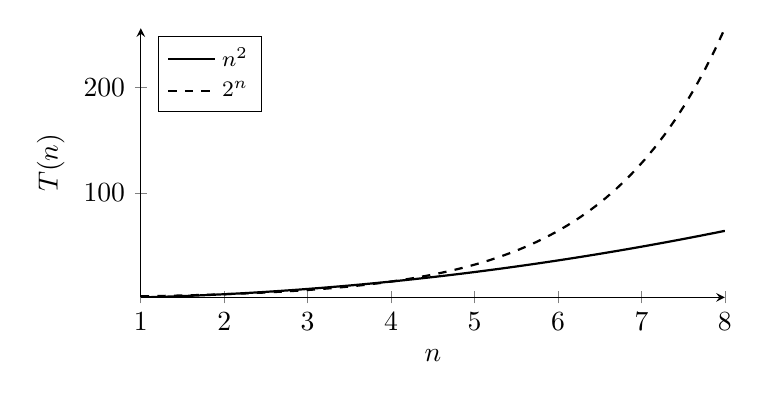
\begin{tikzpicture}
\begin{axis}[width=9cm,height=5cm,xlabel={$n$},ylabel={$T(n)$},
  domain=1:8,samples=60,axis lines=left,
  legend style={font=\footnotesize,at={(0.03,0.97)},anchor=north west}]
  \addplot[thick]{ x^2 };          \addlegendentry{$n^2$}
  \addplot[thick,dashed]{ 2^x };   \addlegendentry{$2^n$}
\end{axis}                         % ← mandatory; the #1 figure-compile bug if missing
\end{tikzpicture}
\end{tikzpic}

% ---- (7) decision tree: per-LEVEL sibling distance (or nodes overlap) ------
% A `child` tree uses ONE sibling distance for all levels by default, so a deep
% node and a shallow leaf collide. Set `level N/.style={sibling distance=…}`
% per level (wider near the root). Hebrew node text in \h{}, math is fine; the
% yes/no edge labels are bare Latin in the LTR `tikzpic` island.
\subsection*{\h{עץ החלטה — מרווח אחים לפי רמה}}
\begin{tikzpic}
\begin{tikzpicture}[every node/.style={font=\small},level distance=15mm,
  level 1/.style={sibling distance=46mm},
  level 2/.style={sibling distance=26mm},
  edge from parent/.style={draw,-{Latex[length=2mm]}}]
\node[draw,rounded corners,fill=cBlueBg] {\h{גיל $>50$?}}
  child {node[draw,rounded corners,fill=cGreenBg] {\h{לחץ־דם $>140$?}}
    child {node[draw,fill=cRedBg]   {\h{סיכון}} edge from parent node[left,xshift=-1mm]{yes}}
    child {node[draw,fill=cGreenBg] {\h{תקין}}  edge from parent node[right,xshift=1mm]{no}}
    edge from parent node[left,xshift=-1mm]{yes}}
  child {node[draw,fill=cGreenBg] {\h{תקין}} edge from parent node[right,xshift=1mm]{no}};
\end{tikzpicture}
\end{tikzpic}

\end{document}
